\documentclass{article}
\usepackage{fullpage}
\usepackage{sectsty}
\usepackage{color}
\usepackage{enumerate}
\usepackage{graphicx, subfigure}
\usepackage{hyperref}
\usepackage{amsfonts, amsmath, amsthm, bm, amssymb}
\usepackage{tcolorbox}
%\usepackage{algorithm}
\usepackage{algorithm2e}
\RestyleAlgo{boxed}% Change from the 'ruled' style to 'boxed'

\usepackage{macro}
\usepackage[utf8]{inputenc}
\usepackage[normalem]{ulem}

\usepackage{centernot}


\newcommand{\defeq}{\mathrel{\mathop:}=}
\newcommand\bigCI{\mathop{\underline{\raisebox{0pt}[0pt][1pt]{$\;||\;$}}}}

\begin{document}

\section*{10-708 Probabilistic Graphical Models}
{\large \bf Homework 2} \hfill {\it Due Mar 21, 11:59 PM}

\noindent\rule{\textwidth}{1pt}

\vspace{5ex}
\subsection*{Rules:}
\vspace{2ex}

\begin{enumerate}
\item Homework is due on the due date at 11:59 PM. The homework should be submitted via \href{https://gradescope.com/courses/14138}{Gradescope}. Solution to each problem should start on a {\it new page} and marked appropriately on Gradescope. For policy on late submission, please see course website.

\item We recommend that you typeset your homework using appropriate software such as \LaTeX. If you are writing, please make sure your homework is cleanly written up and legible. The TAs will not invest undue effort to decrypt bad handwriting.

\item {\bf Code submission:} for programming questions, you must submit the complete source code of your implementation also via \href{https://gradescope.com/courses/14138}{Gradescope}. Remember to include a small README file and a script that would help us execute your code.

\item {\bf Collaboration:} You are allowed to discuss the homework, but you should write up your own solution and code. Please indicate anyone you collaborated with in your submission.

\end{enumerate}

\vspace{7ex}
\noindent\rule{\textwidth}{1pt}

\newpage

%!TEX root = ../main.tex

\section{KL-divergence [30 pts] (Yuanning)}
\subsection{Divergence measures and maximum likelihood estimation (3 + 4 + 4 + 5 = 16 pts)} 
In Lecture 8, we introduced \textit{Iterative Proportional Fitting} (IPF) algorithm as a way to learn the parameters of a undirected graphical model, and we claim that IPF is also a coordinate ascent algorithm (see slide 41). In this question, we are going to prove that \textbf{IPF algorithm is essentially a coordinate ascent algorithm that maximizes the likelihood $p(x; \theta)$ over parameter $\theta$}. Here we consider use KL-divergence as a tool to prove our main result. In Part (a-c) we prove a set of useful lemmas with respect to KL-divergence and MLE. Finally in Part (d), we prove the main result using lemmas from (a-c).

\begin{itemize}
\item[(a)] Let $p(x), q(x)$ be two positive probability densities on $\mathbb{R}$. Prove Gibbs inequality $$D_{KL}\big(p(x) \| q(x)\big) = \int p(x)\log\Big( \frac{p(x)}{q(x)}\Big) dx \geq 0$$ and the equality holds if $p(x) = q(x)$.
\item[(b)] Assume we have $N$ $i.i.d.$ samples $x^{(1)}, ..., x^{(N)} \in \mathbb{R}^d$ from distribution $p(x; \theta^*)$, where $\theta^*$ is the true parameter that we want to estimate. The maximum likelihood estimator is $$\widehat{\theta}_{MLE} \equiv \underset{\theta}{\text{argmax}} ~ \frac{1}{N}\sum_{i=1}^N \log p(x^{(i)}; \theta)$$
Show that, for large $N$, maximum likelihood estimation also (asymptotically) minimizes the KL-divergence $D_{KL}(p(x; \theta^*) \| p(x; \theta))$, i.e. 
$$\widehat{\theta}_{MLE} = \underset{\theta}{\text{argmin}} ~ D_{KL}(p(x; \theta^*) \| p(x; \theta)), ~~~ N \rightarrow \infty$$
\textbf{Hint}: consider the law of large numbers.
\item[(c)] Let $p, q$ be two positive distributions, and $x_A, x_B$ be two (non-overlapping) sets of variables. Prove the following equation $$D_{KL}(p(x_A, x_B) \| q(x_A, x_B)) = D_{KL}(p(x_A) \| q(x_A)) + \sum_{x_{A}}p(x_A)D_{KL}(p(x_B | x_A) \| q(x_B | x_A))$$
\item[(d)] Consider a decomposable undirected graphical model $p(x) = \frac{1}{Z} \prod_i \phi_{C_i}(x_{C_i})$, where $C_1,...,C_k$ are $k$ clusters of the graph, and $U = \cup_{i=1}^k C_i$ is the full set of all nodes. Given a set of $N$ $i.i.d.$ samples $x^{(1)},..., x^{(N)}$, the IPF algorithm estimates the potential function $\phi_C(x_C)$ for each cluster using the following iteration $$\phi_C^{(t+1)}(x_C) = \phi_C^{(t)}(x_C)\frac{\epsilon(x_C)}{p^{(t)}(x_C)}$$
where $\epsilon(x_C) = \frac{1}{N}\sum_{i=1}^{n}\mathbb{I}[x_C = x_C^{(i)}]$ is the empirical marginal distribution of cluster $C$, and $p^{(t)}(x_C) = \sum_{x_{U \setminus C}} p^{(t)}(x) = \sum_{x_{U \setminus C}} \frac{1}{Z^{(t)}} \prod_{i=1}^k \phi_{C_i}^{(t)}(x_{C_i})$ is the estimated marginal distribution of cluster $C$ at the current step $t$. 

Prove that IPF is coordinate ascent in the log likelihood of the data.

\end{itemize}
\textbf{Note}: coordinate ascent is an iterative way to find the maximum of a multivariate function $f(x)$ with $x \in \mathbb{R}^d$. Specifically, at each iteration, it minimizes $f(x)$ over a coordinate $x_i$ or coordinate block $x_C$ ($C = \{i_1,...,i_k\}$ is a subset of all the coordinates) while fixing all the other coordinates $x_{-C}$, i.e. 
$$x_C^{(t+1)} = \underset{x_C}{\text{argmax}} ~f(x_C, x_{-C}^{(t)}) $$


\subsection{Divergence measures and Fisher information (4 + 2 + 4 + 4 = 14 pts)}
Fisher information is a way of measuring the amount of information that an observed variable $x$ has about parameter $\theta$ of a distribution $p(x; \theta)$. Divergence measures, such as KL-divergence, have deep connections to Fisher information from the perspective of information geometry. Here we are going to study some important properties that tie together Fisher information, KL-divergence, and parameter estimation. 
\begin{itemize}
\item[(a)] For a multivariate distribution $p(x; \theta)$ on $\mathbb{R}^d$ with $\theta \in \mathbb{R}^n$, and assume that regularity conditions apply to $p(x;\theta)$, the \textit{Fisher information matrix} $\mathcal{I}(\theta) \in \mathbb{R}^{n \times n}$ is defined as $$\mathcal{I}(\theta) \equiv \mathbb{E}_{p(x;\theta)}\big[ \nabla_{\theta} \log p(x;\theta) \nabla \log p(x;\theta)^T\big]$$ Show that  $$ \mathcal{I}(\theta) = -\mathbb{E}_{p(x;\theta)} [\nabla_{\theta}^2 \log p(x;\theta)]$$ 
\item[(b)] Find the \textit{Fisher information matrix} $\mathcal{I}(\theta)$ for exponential family $p(x;\theta) = h(x)\exp[\theta^TT(x) - A(\theta)]$.
\item[(c)] Let $p(x;\theta)$ be a distribution on $\mathbb{R}$, with $\theta \in \mathbb{R}$, and assume that regularity conditions apply to $p(x;\theta)$. We are often interested in how sensitive the pdf is with respect to parameter $\theta$. Consider distribution $p(x; \theta+\delta)$, where a small perturbation $\delta \in \mathbb{R}$ is added to parameter $\theta$. Show that, for small $\delta$ $$D_{KL}\big(p(x;\theta) \| p(x;\theta+\delta)\big) = -\frac{\delta^2}{2} \mathbb{E}_{p(x;\theta)}\big[\frac{\partial^2}{\partial \theta^2} \log p(x;\theta)\big] + o(\delta^2)$$
\textbf{Note:} here we use little $o$ notation to represent remainder $r = o(\delta^2)$, which means $r / \delta^2 \rightarrow 0$, as $\delta \rightarrow 0$. 
\item[(d)] Now consider the exponential family distribution $p(x;\theta) = h(x)\exp[\theta^TT(x) - A(\theta)]$, and small perturbed $p(x; \theta+\delta)$ with $\theta, \delta \in \mathbb{R}^n$.  Show that $$D_{KL}\big(p(x; \theta)||p(x; \theta+\delta)\big) = \frac{1}{2} \delta^T\nabla^2A(\theta)\delta + o(\|\delta\|^2)$$
\end{itemize}







\newpage
%!TEX root = ../main.tex

\section{CRF Learning for OCR [30 pts] (Yifeng)}

\textbf{Note: Please submit all your answer (including derivations, calculated values, figures) to this problem in the pdf file, the executable code and provided dataset in the *.zip file.}

\subsection{Introduction}
In this problem, you will implement your own code to learn the parameters of a conditional random field (CRF) for optical character recognition (OCR).

In the CRF model, there are two kinds of variables: the hidden variables that we want to model and those that are always observed. In the case of OCR, we want to model the character assignments (such as ‘a’ or ‘c’), and we always observe the character images, which are arrays of pixel values. Typically, the unobserved variables are denoted by $Y$ and the observed variables are denoted by $X$. The CRF seeks to model $P(Y |X)$, the conditional distribution over character assignments given the observed images. We will be working with the OCR model that includes only the singleton and pairwise factors (as we will explain in detail below). The structure of the model is shown below:

\begin{figure}[h]
	\centering
	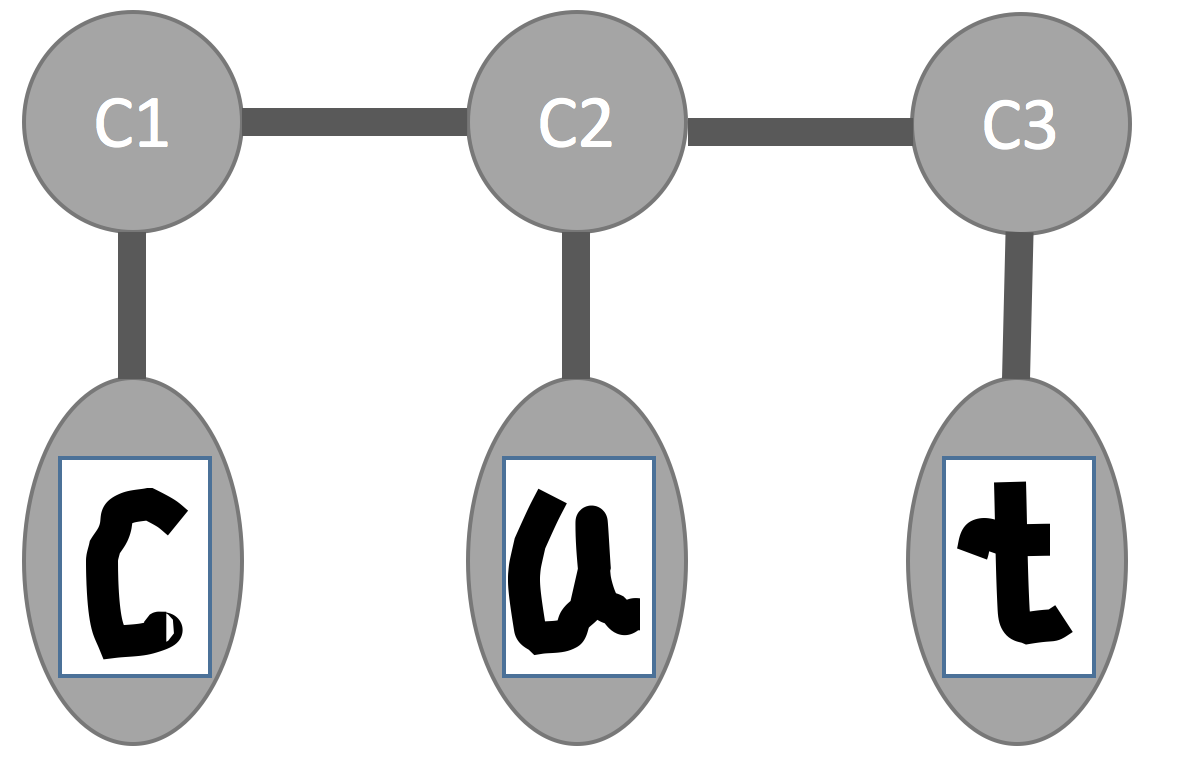
\includegraphics[width = 0.3\linewidth]{figures/figCRF1.png}
	\caption{CRF with singleton and pairwise factors.}
\label{fig:crf}
\end{figure}

As you can see, our CRF for OCR is a specific case of the general CRF mentioned in class. Specifically, you will build the model around log-linear features. A feature is just a function $f_i (D_i)$: $Val(D_i) \rightarrow \mathbb{R}$, where $D_i$ is the set of variables in the scope of the $i$-th feature. Here, all features are binary indicator features (taking on a value of either 0 or 1). Each feature has an associated weight $\theta_i$. Given the features $\{f_i\}_{i=1}^k$ and the weights $\{ \theta_i  \}_{i = 1}^k$, the distribution is defined as:
\begin{align}
P(Y | X; \theta) = \frac{1}{Z_X (\theta)}  \exp \{  \sum_{i=1}^{k} \theta_i f_i (D_i)  \}.
\end{align}
The term $Z_X (\theta)$ is the partition function:
\begin{align}
Z_X (\theta) = \sum_Y \exp \{ \sum_{i=1}^k \theta_i f_i ( D_i )  \}.
\end{align}

In our CRF, we have three types of features:
\begin{itemize}
	\item $f_{i,c}^C ( Y_i )$, which operates on single characters / hidden states (an indicator for $Y = c$).
	
	\item $f_{i,j,c,d}^I ( Y_i, X_{ij})$,which operates on a single character / hidden state and an image pixel	associated with that state (an indicator for $Y_i = c, X_{ij} = d$). These are collectively used to encode the individual probability that $Y_i = c$ given $X_i$.
	
	
	\item $f_{i,c,d}^P (Y_i, Y_{i+1})$which operates on a pair of adjacent characters / hidden states (an indicator for $Y_i = c, Y_{i+1}  = d$).
	
\end{itemize}


\subsection{Gradient of Negative Log-likelihood  [5pts]}

Our goal is to maximize the log-likelihood of the parameters given the data. Thus the cost / loss we minimize is simply the negative log-likelihood, together with a $L_2$-regularization penalty on the parameter values to prevent overfitting. The function we seek to minimize is:
\begin{align}
\text{nll} (X, Y, \theta) = \log(Z_X(\theta))  - \sum_{i =1}^{k} \theta_i f_i (Y, X) + \frac{\lambda}{2} \sum_{i = 1}^{k} \theta_i^2.
\end{align}

\textbf{Question: }Please prove that partial derivatives for this function have an elegant form:
\begin{align}
\frac{\partial }{\partial \theta_i} \text{nll} (X, Y, \theta) = E_{\theta} [ f_i ] - E_D [ f_i] + \lambda \theta_i,
\end{align}
where
\begin{align}
E_{\theta} [f_i] &= \sum_{Y'} P( Y' | X) f_i (Y', X), \\
E_D [ f_i ] &= f_i (Y, X).
\end{align}
We drop the $\theta$ from $P(Y' | X)$ for convenience.


\subsection{Shared Parameters [2pts]}

There is one more detail to take care of: shared parameters across multiple features. Parameter sharing is a form of templating used to reduce the total number of parameters we need to learn. Let $\{f^{(i)}  \}$ be the set of features that share parameter $\theta_i$. 

\textbf{Question: }Give a brief explanation that we can expend the equations (3, 4) above as:
\begin{align}
\text{nll} (X, Y, \theta) = \log ( Z_X (\theta) ) - \sum_{i=1}^{k} \theta_i (  \sum_{f_j \in \{ f^{(i)} \} }  f_j (Y, X ) ) + \frac{\lambda}{2} \sum_{i = 1}^k \theta_i^2.
\end{align}
\begin{align}
\frac{\partial }{\partial \theta_i} \text{nll} (X, Y, \theta) =  \sum_{ f_j \in \{ f^{(i)}   \}   } E_{\theta} [ f_j ] - \sum_{  f_j \in \{ f^{(i)}  \}  }  E_D [ f_i] + \lambda \theta_i.
\end{align}
Note that in this case, $\theta_i$ is not necessarily related to $f_i$ any longer. Instead, $\theta_i$ is associated with a set of features $\{ f^{  (i)  }  \}$. $k$ is the total number of parameters of $\theta_i$, and not necessarily the total number of features $f_j$. The parameters that we use in the CRF are:
\begin{itemize}
\item $\theta_c^C$, shared by $ \{  f_{i,c}^C (  Y_i  )    \}_i   $.

\item $\theta_{c,d}^I$, shared by $ \{   f_{i,j,c,d}^I  (  Y_{i}, X_{ij}   )          \}_{i,j}       $.


\item $\theta_{c,d}^P$, shared by $ \{   f_{i,c,d}^P (Y_i, Y_{i+1})      \}_i  $.
\end{itemize}
Essentially, this parameter tying scheme ties parameters across different locations together; that is, a character at the start of the word shares the same parameters as a character at the end of the word.


\subsection{InstanceNegLogLikelihood Implementation [18pts]}

Given this discussion, we can now state your mission: for a given data instance $(X,Y)$ and a parameter setting $\theta$, you must compute the cost function (regularized negative log-likelihood) and the gradient of parameters with respect to that cost. Doing so involves six terms (ignoring the issue of shared parameters in these):

\begin{itemize}
\item The log partition function: $\log ( Z_X (\theta) )$

\item The weighted feature counts: $\theta_i f_i ( Y, X )$

\item The regularization cost: $ \frac{\lambda}{2} \sum_{i=1}^k \theta_i^2$

\item The model expected feature counts: $\sum_{Y'}  P(Y' | X) f_i (Y', X) $

\item The data feature counts $f_i (Y, X)$

\item The regularization gradient term: $\lambda \theta_i$.

\end{itemize}

In this problem, you are provided with a single instance and related parameters in \verb|q2instance.mat| to help you implement your \verb|InstanceNegLogLikelihood| function, which should return the negative log-likelihood and gradient of the parameters. First, we should clarify what exactly we mean by a data “instance.” The input to \verb|InstanceNegLogLikelihood| function includes $X$ and $Y$ which together form a single instance $(X,Y)$. This instance corresponds to one
word, that is, a sequence of characters.

Thus, the variable $Y$ is a vector of character values. For example, $Y = (3, 1, 20)$ means that this instance contains the word “cat.” The variable $X$ is a matrix where the $i$-th row contains the pixel values for the ith character in the example. Each row has 32 values, since the images are 8x4 pixels. The feature sharing described above comes into play due to the fact that our data instances are not single images (as they were in the first part of the assignment) but instead sequences of images that we want to consider together.


\subsubsection*{(a) Number of Parameters [6pts] }

\textbf{Question:} Since we have a sequence of $Y$ with length 3, where each position has 26 hidden states; and each image has 32 binary positions. Considering the shared parameters across multiple features, show that $\theta$ has length of $2366$, i.e., clarify how many specific parameters in three different cases: $\theta_c^C, \theta_{c,d}^I, \theta_{c,d}^P$.

%26 + 26*26 + 26*(32*2) 
%each pixel has two states


\subsubsection*{(b) Implementation of InstanceNegLogLikelihood [12pts]}

Please implement your \verb|InstanceNegLogLikelihood| function:

\verb|[nll, grad] = InstanceNegLogLikelihood(X, y, theta, params)|.

\textbf{Question:} You are required to provide the following values in your pdf report:
\begin{itemize}
\item  \verb|sampleNLL|:  $\log ( Z_X (\theta) ) - \sum_{i=1}^{k} \theta_i (  \sum_{f_j \in \{ f^{(i)} \} }  f_j (Y, x ) ) + \frac{\lambda}{2} \sum_{i = 1}^k \theta_i^2$,

\item  \verb|sampleGrad(1:5)|: $\sum_{ f_j \in \{ f^{(i)}   \}   } E_{\theta} [ f_j ] - \sum_{  f_j \in \{ f^{(i)}  \}  }  E_D [ f_i] + \lambda \theta_i$,
\end{itemize}
where
\verb|[sampleNLL, sampleGrad] = InstanceNegLogLikelihood(sampleX, sampleY, sampleModelParams)|, and \verb|sampleX|, \verb|sampleY|, \verb|sampleTheta|, \verb|sampleModelParams| from \verb|q2instance.mat|:
Feel free to use any programming language you want and any resources from the Internet as soon as you acknowledge them properly.

% sampleNLL: 9.7743
% sampleGrad: [-0.8846         0   -0.9231    0.0385   -0.9231]



\subsection{Stochastic Gradient Descent [5pts]}

In this question, we want to train the CRF using stochastic gradient descent with vanishing step size.

In \verb|q2dataset.mat|, we provide \verb|trainData| and \verb|testData|. Each is a struct array with $X$ and $y$ fields. In both, each $(X, y)$ pair is the input the \verb|InstanceNegLogLikelihood|: $X$ gives the observations and $y$ gives the labels. You can directly use \verb|sampleModelParams| from \verb|q2instance.mat| as hyperparameters for training, and use \verb|sampleTheta| from \verb|q2instance.mat| for initialization of parameters.

\textbf{Question:} Train the model using stochastic gradient descent, plot the test loss versus training steps evaluated on the first 10 samples in the \verb|testData|. We only require you to train the model for one epoch (i.e., 220 steps in total), since the training is time consuming. We recommend using the learning rate of $\alpha_k = \frac{1}{1 + 0.05k}$, where $k$ is the number of steps.




\newpage
%!TEX root = ../main.tex
\newcommand\independent{\protect\mathpalette{\protect\independenT}{\perp}}
\def\independenT#1#2{\mathrel{\rlap{$#1#2$}\mkern2mu{#1#2}}}

\section{Hierarchical Mixture of Experts [40 pts] (Xiongtao)}

\noindent
In this problem, we are going to work with a two-level hierarchical mixture of experts network (HME). Let
$\xv \in \Rb^{r}$ is the input, $\yv\in \Rb^{s}$ is the output. If $\yv$ is defined in a continuous space, it is a regression problem, and if $\yv$ is defined in categories, it is a classification problem. The dataset consists of $T$ paired observations $\Xc = \{(\xv^{(t)}, \yv^{(t)})\}$, where $t=1, ..., T$. Here we are going to use HME to work on regression problems.

The basic structure of an HME is shown in Figure \ref{fig:hme}. An HME is a tree in which non-terminals are gating networks and leaf nodes are expert networks. Both gating networks and expert networks use $\xv$ as input. Usually, expert networks and gating networks are modeled as generalized linear model (GLM). Expert networks consist of some simple models, i.e. linear regression (for regression), Bernoulli probability model (for classification) and so on. Each of them produces a variable $\muv_{ij}$ for each input vector. Gating networks consist of distributions that generate a partition of unity at each point in the input space, for example, they could be softmax operations on $\xv$. Intuitively, expert networks define the relationship between observation and response, while gating networks act as prior/weights for expert networks, determining which expert networks are going to make a decision about $\xv$. Because gating networks also depend on data, there would various combinations of expert networks used for decisions for different $(\xv, \yv)$. Therefore, HME can model complex data by the combination of some simple models. 
	
\begin{figure}[!ht]
	\centering
	% Requires \usepackage{graphicx}
	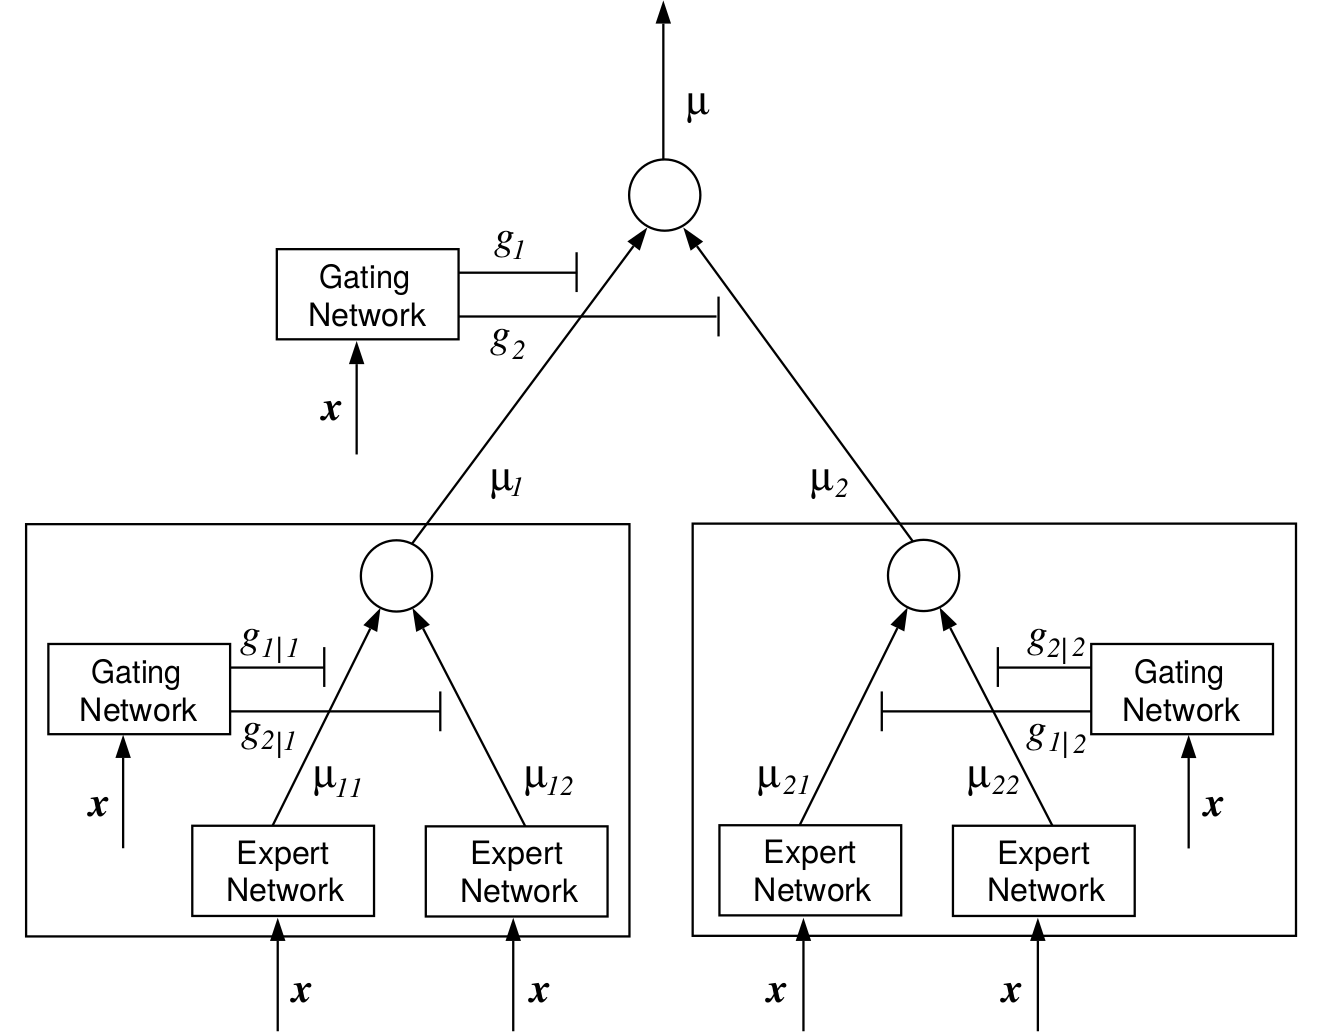
\includegraphics[width=0.6\textwidth]{figures/2_layer_HME.png}\\
	\caption{A two-level hierarchical mixture of experts.}
	\label{fig:hme}
\end{figure}


In the HME, there are $MN> 0$ expert networks in the bottom layer, we use $ENet_{ij}$ to represent expert networks with index $i, j$, $i=1:M$, $j=1:N$. All $ENet_{ij},~j=1:N$ are children of $i-th$ node in the middle layer of the tree. Here, the expert networks are defined as linear regression models, with 
$$\muv_{ij} \sim \Nc(\Uv_{ij}\xv, \sigma_{i}^2\Iv)$$
where $\sigma_i$ is shared among $i-th$ block of expert networks $ENet_{ij}\quad j=1,...,N$, $\Uv_{ij}$ is the weight matrix, and $\Iv$ is the identity matrix. 

For the gating network in the top level, it is a "softmax" function of $\vv_{i}\xv$ as
$$g_{i} = \frac{e^{\vv_{i}^T\xv}}{\sum_{i'}e^{\vv_{i'}^T\xv}}$$
where $\vv_{i}$ is a weight vector, $i=1:M$. Clearly, $g_i$ is a GLM for $\xv$. 

For gating network in the lower level, we also define them as a GLM of $\xv$, as

$$g_{j|i}(\xv) = \frac{e^{\vv_{ij}^T\xv}}{\sum_{k}e^{\vv_{ik}^T\xv}}$$
where $j=1:N$.  

As we mentioned before, gating networks could be viewed as weight of each node. Therefore, the output vector at each non-terminal node of the tree is the weighted output of the experts below that node, i.e. for $i-th$ node in the middle layer, the output is
$$\muv_i = \sum_j g_{j|i}\muv_{ij}$$
and the output at the top level is:
$$\muv = \sum_i g_i\muv_i$$


Finally, we define the response variable $\yv$ as a (conditional) linear regression on the output of each expert network $\muv_{ij}$ as 
$$P(\yv|\muv_{ij}, \sigma) = \Nc(\muv_{ij}, \sigma^2I)$$ 
Where $\sigma$ is the standard deviation, which is shared for the whole network. 

From another point of view, we treat the gating networks as prior for $\yv$ and the expert networks as conditional distribution with data, then we can get the distribution as
$$P(\yv, \muv|\xv, \thetav) = \sum_{i}g_i(\xv, \vv_{i})\sum_{j}g_{j|i}(\xv, \vv_{ij})P(\yv|\muv_{ij}, \sigma)P(\muv_{ij}|\xv, \sigma_{i})$$
where $\muv = \{\muv_{11}, ..., \muv_{MN}\}$, and $\thetav$ represents all parameters in the network, i.e. for both expert networks and gating networks.

We can also define a posterior probability associated with each node, that reflects the extent to which the node is activated. For the top level nodes, using the Bayes Rule, we define the posterior probabilities as 
$$h_{i} = \frac{g_{i}\sum_{j}g_{j|i}P_{ij}(\yv|\xv, \theta)}{\sum_{i}g_{i}\sum_{j}g_{j|i}P_{ij}(\yv|\xv, \theta)}$$
where $$P_{ij}(\yv|\xv, \thetav_E) \defeq \sum_{\muv_{ij}}P(\yv|\xv, \muv_{ij}, \sigma)P(\muv_{ij}|\xv, \sigma_{i})$$
which is the factorized distribution associated with each expert network, and $\thetav_E$ represents all parameters associated with expert networks, i.e. $\thetav_E = \{\sigma_i,~i=1:M\} \cup \{\sigma\}\cup\{\Uv_{ij},~~ i=1:M, ~~j=1:N \}$.

\subsection*{3.1. Warm up [2 + 1 + 1 = 4 pts]}

\begin{enumerate}
\item a problem in the model is that there are latent variables $\muv$ in the full distribution, which complicate the model. Therefore, we would like to marginalize out $\muv$ first. Please derive $p(\yv|\xv, \theta)$. You can keep $g_{i}$ and $g_{j|i}$ in the distribution, and just work with other parts of the distribution. In the later part of the question, we will just use the marginal distribution, therefore, please be careful and make sure your derivation is correct. 

Hint: Linear Gaussian system would be helpful here.

\item Write out the posterior distributions at the nodes in the bottom level of the network, that is, $h_{j|i}$. 

\item HME is considered as a nonlinear model for $\xv$ and $\yv$, reasoning why this network is a nonlinear model.  

\end{enumerate}


\subsection*{3.2. EM algorithm for HME [19 pts]}

To derive the EM algorithm, we first define binary latent variables $z_i$ and $z_{j|i}$ that associate with the nodes in the network. $z_{j|i}=1$ means expert network $ENet_{ij}$ is activated, $z_i=1$ means node $i$ in top layer is activated. For the bottom layer, we only allow one expert network for the children of $i-th$ node in the top layer being activated, that is $\sum_{j}z_{j|i} = 1$, and we also just allow one node in the top level activated, that is, $\sum_{i}z_i=1$. We define $z_{ij}= z_{i}z_{j|i}$, which could be interpreted as the activation of the specific expert network.

With $z_i$ and $z_{j|i}$, we could rewrite the distribution for a single data point as
$$P(\yv, \zv|\xv, \thetav) = \prod_{i}\prod_{j}(g_i g_{j|i}P_{ij}(\yv|\xv,\thetav))^{z_{ij}}$$
where $\zv =\{z_{ij}\},~i=1:M,~j=1:N$. 

Note, $z_{ij}$ is associated with each data point, then the complete-data distribution among $T$ data points is
$$P(\Yv, \Zv|\Xv, \thetav) = \prod_{t}\prod_{i}\prod_{j}(g_ig_{j|i}P_{ij}(\yv^{(t)}|\xv^{(t)},\thetav))^{z^{(t)}_{ij}}$$

where $\Yv = \{\yv^{(1)}, ..., \yv^{(T)}\}$, and $\Zv = \{z^{(t)}_{ij} \},~i=1:M,~j=1:N,~t=1:T$. 

Then, the EM algorithm could be applied based on the distribution above. Below we provide the pseudo-code for the algorithm. 

\begin{algorithm}[H]
	\SetAlgoLined
	\SetKwInOut{Input}{Input}	
	\SetKwInOut{Output}{Output}
	\Input{$\Xc$, $M$, $N$, MaxIter, and other optional parameters}
	\Output{Parameter $\thetav$, Log-likelihood in the update, Fitted output $\hat{\Yv}$, $\Eb[z_{ij}^{(t)}|\Xc]$ in the last iteration}
	\BlankLine
	Initialize parameters $\thetav$\;
	\BlankLine
	\tcp{Compute Log-likelihood}	
	Compute and record log-likelihood with initial parameters
	\BlankLine
	\For{$k\leftarrow 1$ \KwTo MaxIter}{
		\tcp{Stage 1: E-Step}		
		Update $\Eb[z_{i}^{(t)}|\Xc]$, $\Eb[z_{j|i}^{(t)}|\Xc]$ and $\Eb[z_{ij}^{(t)}|\Xc]$
		\BlankLine
		\tcp{Stage 2: M-Step}
		\tcp{Update $\Uv_{ij}$}
		For each expert $(i,j)$, update $\Uv_{ij}$ by directly solving MLE
		\BlankLine
		\tcp{Update $\sigma_i$}
		For each $i$, update $\sigma_{i}$ by directly solving MLE 
		\BlankLine		
		\tcp{Update $\sigma$}
		Update $\sigma$ by directly solving MLE 		
		\BlankLine		
		\tcp{Update $\vv_i$ in top-level gating network}
		For each top-level gating network, solve an iteratively reweighted least squares (IRLS) problem to update
		 $\vv_i$
		\BlankLine		 
		\tcp{Update $\vv_{ij}$ in lower-level gating network}
		For each lower-level gating network, solve an IRLS problem to update $\vv_{ij}$
		\BlankLine		
		\tcp{Stage 3: Report Log-likelihood}	
		Compute and record log-likelihood				
	}
	\tcp{Compute the prediction of $\yv$}
	Compute the fitted output $\hat{\Yv}$ for all observations $\Xv$
\caption{Pseudo-code of EM algorithm for HME model}
\label{alg:em}
\end{algorithm}

\subsubsection*{a. E-step [3 + 1 = 4 pts]}
\begin{enumerate}
	\item Derive E-step, that is, derive $\Eb[z_{i}^{(t)}|\Xc]$, $\Eb[z_{j|i}^{(t)}|\Xc]$ and $\Eb[z_{ij}^{(t)}|\Xc]$, you don't need to spread out $g_i$, $g_{j|i}$ and $P_{ij}$. 
	\item What is the relationship between $\Eb[z_{i}^{(t)}|\Xc]$, $\Eb[z_{j|i}^{(t)}|\Xc]$, $\Eb[z_{ij}^{(t)}|\Xc]$, and posterior distributions of nodes, as derived in Part 3.1.3?
\end{enumerate}


\subsubsection*{b. M-step [3 + 6 + 4 = 13 pts]}

\begin{enumerate}
\item write down the problems you need to solve to update parameters (the parameters you need to optimize), you don't need to spread out $g_i$, $g_{j|i}$ and $P_{ij}$, but please be as specific as possible, that is, throw out constant terms with respect to each parameter as much as possible, for example, parameter $\Uv_{ij}$ is only related to $\Eb[z_{ij}^{(t)}|\Xc]$ and $P_{ij}(\yv^{(t)})$, $t=1:T$. 

\item Derive the updating rules for parameter in expert networks based on the problem you write in last question (3.2.b.1). As indicated in the algorithm, we can directly solve the MLE to get the update rules. More specifically, derive updating rules for $\Uv_{ij}$, $\sigma_i$ and $\sigma$, where $i=1:M$, $j=1:N$. The result should be as specific as possible, that is, they could be directly used in the implementation.  

\item We need to update $\vv_i$ and $\vv_{ij}$ using the IRLS algorithm. Based on the problems in previous part, derive the IRLS updating rules for $\vv_i$ and $\vv_{ij}$ for $i=1:M$, $j=1:N$. The result should be as specific as possible, that is, they could be directly used in the implementation.  
\end{enumerate}

\subsubsection*{c. Log-likelihood and prediction [2 pts]}
\begin{enumerate}
\item To monitor the progress and evaluate the performance of the algorithm, we need to report the log-likelihood in each iteration and calculate the prediction in the end. Write out the expressions of log-likelihood and prediction. You can use $g_i$, $g_{j|i}$ and $P_{ij}$ in the expression, if any of them are in the expressions. But please be as specific as possible, that is, they could be directly used in the implementation.  
\end{enumerate}

\subsection*{3.3. Implementation of EM algorithm [17 pts]}

In this part, we are going to implement EM algorithm. Please implement the algorithm in the notebook $Question\_3.3.ipynb$ and answer some following questions. You may follow Algorithm \ref{alg:em} in your implementation. \emph{In your submission, please print out the notebook as a PDF file and put the PDF file as part of the homework, in the mean time, please also submit the raw jupyter notebook file with filename $Question\_3.3\_yourandrewid.ipynb$.}\\

\noindent
\textbf{Hint: the problem is designed based on the paper Jordan \& Jacobs et al. 1994 \cite{jordan1994hierarchical}. You may get some ideas of how to solve the problem by reading the paper. }

\bibliography{references}





\newpage
%!TEX root = ../main.tex

\section{Logistic Regression [Bonus: 1 + 3 + 1 + 5 = 10 pts] (Yuanning)}
\textcolor{red}{(\textbf{Note: This is a bonus problem that is optional.})}

Logistic regression is a specific case of generalized Iinear model to model joint distribution between $(y, x)$, with conditional distribution $y|x \sim \text{Bernoulli}(\mu)$, and logit link function $\beta^Tx = \log\Big(\frac{\mu}{1-\mu}\Big)$. In this problem, we'll use logistic regression to classify a person's age group (under 40 or not) from his movie ratings. Given $n$ $i.i.d.$ samples $(y_1, x_1), ..., (y_n, x_n)$, we formulate the problem as a binary classification with output label  $y \in \{0,1\}^n$, corresponding to whether a person`s age is under $40$, and input features $X \in \mathbb{R}^{n \times (p+1)}$. The first column of $X$ is taken to be $1_n$ to account for the intercept term. we solve the logistic regression problem using Iteratively Reweighted Least Squares (IRLS).

\begin{enumerate}
\item[(a)] Find the log likelihood of the samples $\ell(y, X, \beta)$.
\item[(b)] Assume a fixed step length $t = 1$, derive the IRLS update for $\beta$. 
\item[(c)] Given $X$, $y$ and $t$, write out the steps for performing IRLS to estimate $\hat{\beta}$.
\item[(d)] Now, implement IRLS using the movie data set on the website (in \texttt{Question4\_data.zip}). You can stop IRLS when the change between consecutive objective values is less than 1e-6. Report both the train and test errors of classifying whether a person is under $40$. Plot $f^{(k)}$ versus $k$,  where $f^{(k)}$ denotes the objective value at outer iterations $k$ of IRLS. 
\\
\textbf{Note:} 
\begin{itemize}
\item As for the step size, the pure Newton`s method uses $t = 1$.  However, in practice we often use damped Newton`s method $x^+ = x - t(\nabla^2f(x))^{-1}\nabla f(x)$. At each Newton step, the step size $t$ is typically chosen by using backtrack line search, with parameter $0 < a \leq 0.5$, and $0 < b < 1$. At each iteration, we start with $t = 1$, and while $$f(x + tv) > f(x) + at\nabla f(x)^Tv $$ we shrink $t \leftarrow bt$, otherwise we perform the Newton update with the current $t$. Note that $v = -(\nabla^2f(x))^{-1}\nabla f(x)$ is the Newton direction.
\item Initialize your weights with zeros. 
\item Feel free to use Python/Matlab or any other language for your implementation. 
\item Please submit all your answer (including derivations, calculated values, figures) to this problem in the pdf file, the executable code and provided dataset in the *.zip file.
\end{itemize}
\end{enumerate}

%\bibliography{references}
\bibliographystyle{unsrt}


\end{document}
